% This file was created by tikzplotlib v0.9.8.
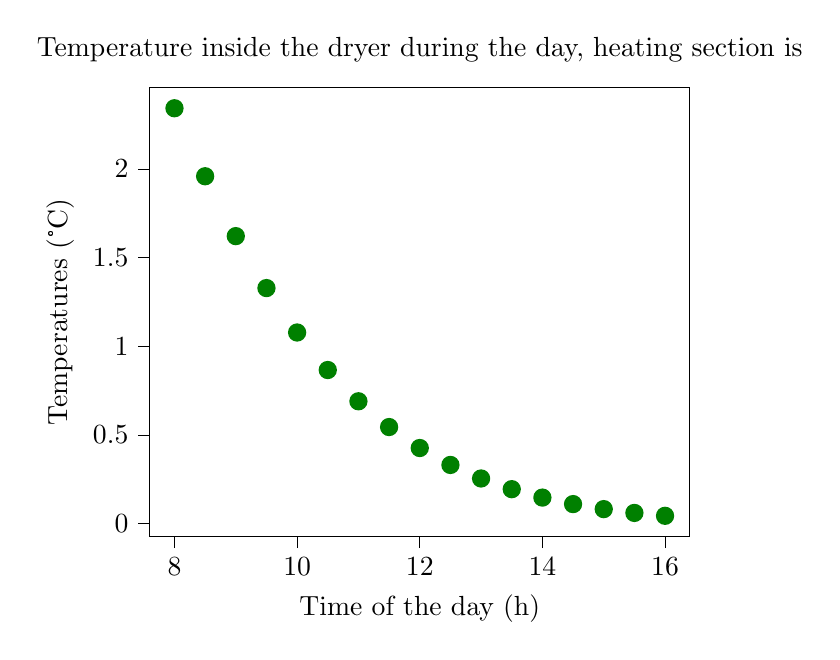
\begin{tikzpicture}

\begin{axis}[
tick align=outside,
tick pos=left,
title={Temperature inside the dryer during the day, heating section is},
x grid style={white!69.0196078431373!black},
xlabel={Time of the day (h)},
xmin=7.6, xmax=16.4,
xtick style={color=black},
y grid style={white!69.0196078431373!black},
ylabel={Temperatures (°C)},
ymin=-0.0720661228058306, ymax=2.45716357853655,
ytick style={color=black}
]
\addplot [semithick, green!50!black, mark=*, mark size=3, mark options={solid}, only marks]
table {%
8 2.3421985921119
8.5 1.95858907703574
9 1.62083637295037
9.5 1.3277543903576
10 1.07704457030553
10.5 0.865447024633353
11 0.68907873520463
11.5 0.543771467177797
12 0.425346765053288
12.5 0.329814066720256
13 0.253497900030204
13.5 0.193107333206422
14 0.145762131980755
14.5 0.108988717305379
15 0.0806966913132008
15.5 0.059144265326013
16 0.0428988636188231
};
\end{axis}

\end{tikzpicture}
